\documentclass[a4paper, 12pt]{report}
\renewcommand{\tiny}{\normalsize}
\renewcommand{\footnotesize}{\normalsize}
%\renewcommand{\small}{\normalsize}
%\renewcommand{\large}{\normalsize}
%\renewcommand{\Large}{\normalsize}
%\renewcommand{\LARGE}{\normalsize}
%\renewcommand{\huge}{\normalsize}
%\renewcommand{\Huge}{\normalsize}
\usepackage{fancyhdr,blindtext}
\pagestyle{fancy}
\usepackage{enumitem}
\usepackage{graphicx} 
\usepackage{caption} 
\usepackage{subcaption} 
\usepackage{parskip}
\setlength{\parindent}{15pt}
\usepackage[margin=0.75in]{geometry}
\usepackage{listings}
\usepackage{amsmath}
\usepackage{hyperref}
\graphicspath{ {images/} }
\usepackage{float}
\usepackage{longtable}

\lstset{
	frame=single,
	breaklines=true
	columns=flexible
	keepspaces=true
}
\lstdefinestyle{myCustomPythonStyle}{
	language=R,
	numbers=left,
	stepnumber=1,
	numbersep=10pt,
	tabsize=5,
	showspaces=false,
	showstringspaces=false
}


\begin{document}
\begin{titlepage}
	\centering
	{\scshape\LARGE University of California, Davis \par}
	{\scshape\Large STA160 Project Report\par}
	\vspace{5cm}
	
	
	{\huge\bfseries Identify Fake Users on Twitter \par}
	\vspace{3cm}
	
	{\Large Guanyu Chen \par}
	{\large\itshape SID: 999329481 \par}
	
	{\Large Jieyi Chen \par}
	{\large\itshape SID: 999823783 \par}

	{\Large Tongke Wu\par}
	{\large\itshape SID:914478812 \par}
		\vfill
% Bottom of the page
	{\large \today\par}
\end{titlepage}

\section*{ABSTRACT}
Twitter has become a popular social network tool to interact with people and spread the news. However, a large number of fake/spam users are actively and intentionally generating certain information to influence the on-line community or generate profits. Therefore, it is essential to detect the fake/spam accounts in order to maintain and optimize the Twitter users' experience. \par

\noindent In this project, we used 47 features to depict the Twitter users' behaviors and developed Random Forest, Logistic Regression and Support Vector Machine models based on these information to discriminate the fake/spam accounts from the genuine.
 
\section*{INTRODUCTION}
As Twitter rapidly grows, a large number of fake/spam accounts infiltrate into the social network. According to a study conducted by the University of Southern California and Indiana University\footnote{O.Varol, E.Ferrara, C.A.Davis, F.Menczer, and A.Flammini. Online Human-Bot Interactions: Detection, Estimation, and Characterization}, there are approximately 9 - 15\% Twitter's monthly active users are bots, which are around 28.9 million to 47.9 million potential fake users. We believe that these accounts can potentially lead to the following three severe negative consequences.

\begin{enumerate}
	\item \textbf{Misleading Propagandas:} Certain individuals or organizations might hire these bots to spread misleading news to influence the public. This act can significantly influence the genuine users' experience because they are exposed to a great deal of fraudulent information.
	\item \textbf{Leak of Personal Information:} The fake accounts often generate many urls to redirect other users to the fishing websites, which might potentially cause these users to leak their personal information and suffer from financial losses 
	\item \textbf{Intrusive Advertisement:} Potential advertisers might choose to hire the computer-generated bots instead of using the Twitter platform to promote their products because it is less expensive and effective

\end{enumerate}
Therefore, Twitter needs effective detection models to purify the on-line community and improve the user experiences. This optimization will potentially bring Twitter more revenue through advertisements and increase its reputation in the public.


\section*{DATA}
\subsection*{Source:}
\textbf{Labeled Twitter User Account:} We labeled the twitter accounts into the following categories:
\begin{enumerate}
	\item Genuine users: verified accounts that are human-operated
	\item Social spambots: retweeters of political candidates, spammers of paid apps for mobile devices and products on sales for e-Commerce sites
	\item Traditional spambots: spammers of scam URLs and job offers	
	\item Fake users: accounts that are used to inflate the number of followers of another account
\end{enumerate}
We acquired the genuine users, social spambots and traditional spambots' information from \href{http://mib.projects.iit.cnr.it/dataset.html}{My Information Bubble}. The fake users' info are brought from \href{https://www.fastfollowerz.com/closed/}{Fast Followerz}, an on-line company that generates accounts to add followers to a designated user. \par

\noindent\textbf{User Profile Information and Tweets:} We used the user ids provided by the sources above to acquire the most recent user profile info, tweets and followers/followings data from the Twitter API.

\subsection*{Limitation}
\begin{enumerate}
	\item Some of the fake accounts provided by MIB are related to specific categories. For example, parts of the social spambots users are the retweeters of an Italian political candidate. Therefore, these accounts might share similar contents and characteristics.
	\item We were restricted by the Twitter API's rate limits where we can only make certain number of requests per 15 minute periods. In addition, as we tried to request more data, the number of successful requests had kept decreasing and sometimes the API did not return all the info that we requested. Lastly, we found that we could only retrieve a maximum number of 3,200 possible tweets per user. 
	
\end{enumerate}

\section*{METHODOLOGIES}
\subsection*{Feature Engineering}
Although Twitter has attempted to filter the fake/spam users from its community, these accounts still keep evolving and they are even trying to develop new tactics to evade from the existing detection tools. Therefore, it is challenging to apply the appropriate features to capture the patterns of their behaviors. \par

\noindent We had discovered that the fake users tend to follow a large number of people who are not within their friends' circle. The spammers, such as the advertisement spambots, are very likely to produce similar content with high frequency. Therefore, we did not only use the data that we got from the API, but also generated effective features by referencing the methods that other studies had created to depict the fake users' behaviors.

\subsection*{Classifiers}
\subsubsection*{Random Forest}
Random Forest is a supervised machine learning technique for classification and regression. In this project, we will specifically use it to perform the classification tasks because we wanted to predict whether the twitter account is genuine or fake. \par

\noindent Random Forest is one of the most accurate classifier available that can perform well even with missing or unbalanced datasets. It can accurately identify the important variables without deletion even with thousands of input variables. Moreover, it will output the importances of predictive variables in the model. \par

\noindent However, this model might over-fit the datasets and be biased toward the categorical variables with different number of levels. In addition, we have very little control of it because we can only tune the parameters and the random seeds.

\subsubsection*{Logistic Regression}
Logistic regression belongs to the family of exponential or log-linear classifiers. First, it extracts some sets of weighted features from the input variables, then, it takes the logs and combines them linearly. In other words, each feature is multiplied by a weight score and the model aggregates the results. Logistic regression is used to separate an observation into two classes and multinomial logistic regression divides the data into more than two classes. But in general, we referenced all of them as logistic regression despite the number of classes that we try to categorize the data into. \par

\noindent Sometimes, logistic regression can be overfitting. If a feature can perfectly predict the outcome for a training set, it might because the model assigns a high weight to this variable. It attempts to perfectly fit all the details of the dataset. This situation can also happens if the factor correlates with the predictive class. Overfitting can cause the model not be general enough to predict well on other datasets. 


\noindent Therefore, there are two common regularization terms called **L1** and **L2** to avoid overfitting:

\noindent \textbf{L1} regularization is a linear function of the weight values, named after the L1 norm $|w|$, the sum of the absolute values of the weights. \\
\textbf{L2} regularization is called ridge regression, which is the sum of the square of the weights $||w||$.\\

\noindent\textbf{The LogisticRegression in sklearn:}
Logistic regression is also known as logit regression, maximum-entropy classification (MaxEnt) or the log-linear classifier. In this model, the probabilities of describing the possible outcomes of a single trial are modeled using a \href{https://en.wikipedia.org/wiki/Logistic_function}{logistic function} \par

\noindent To optimize the problem, we need to minimize

$$
f(x) = \frac 1 {1+e^{-x}}
$$

\noindent L1 regularized logistic regression solves the following optimization problem:
$$
min\frac1{2}w^Tw + C \sum_{i = 1}^n log(exp(-y_{i}(X_{i}^Tw + c)) + 1)
$$

\noindent L2 penalized logistic regression minimizes the following cost function:

$$
min\frac1{2}||w||_{1} + C \sum_{i = 1}^n log(exp(-y_{i}(X_{i}^Tw + c)) + 1)
$$

\subsubsection*{Support Vector Machine}
As ordinary discriminative classifiers, Support Vector Machine
takes in labeled training data and then outputs an optimal hyperplane that categorizes new examples. Especially in the non-separable cases, SVM is able to draw nonlinear boundaries among the classes. It aims to optimize
$$min_{\beta, \beta_0}\frac{1}{2}||\beta||^2+C\sum_{i=1}^{N}\xi_i$$ 
$$subject\ to\ \xi_i\geq 0,\ y_i(x_i^T\beta+\beta_0)\geq 1-\xi_i\ \forall i$$ 
where $C$ is the penalty/cost, $\xi_i$ are slack variables. The value $xi_i$ in the constraint is the proportional amount by which the prediction $f(x_i)=x_i^T\beta+\beta_0$ is on the wrong side of its margin.\\

\noindent SVM is robust in high dimensional spaces and can still work well when the dimension of the features is larger than the sample size. In addition, different kernal functions can be assigned to the decision function so that the nonlinear relation can be satisfied.\\
In our project, we used rbf kernel and linear kernel as following
\begin{enumerate}
	\item []linear:\ $<x,x^{'}>$
	\item []rbf:\ $exp(-\gamma|x-x^{'}|^2)$
\end{enumerate}

\section*{ANALYSIS}
In order to mimic the approximate proportion of fake/spam users in reality, we randomly selected accounts from our original dataset and made sure that 10.78\% of each sample dataset are fake users. We also generated three other dataset for further validation and one of the four has genuine to fake ratio of 3:1 because we wanted to check whether the proportion of the accounts plays a role in the model accuracy. 

\subsection*{Feature Exploration}
Inspired by other papers, we created 47 features and categorized them into the following categories: profile features, content features, behavior features and graph features. Table 1 briefly describes the definition of each feature. \par

\begin{table}[H]
	\captionof{table}{Features Category} \label{tab:title} 
	\begin{center}
		\begin{tabular}{p{4.5cm} | p{11cm}}
			\hline
			Name & Description \\
			\hline
			\multicolumn{2}{|l|}{Profile Features} \\
			\hline
			status count & the number of total tweets \\
			followers/friends count& the number of followers/followings \\
			favorites count & the number of likes receives\\
			fo-fo ratio & the ratio of followers count to friends count \\
			age & the duration that the account has existed \\
			reputation & the ratio of followers count to the sum of followers and friends\\
			description & the words count of individual description on personal website \\
			account setting & the basic settings of an account, such as default image, notification on-off  \\
			\hline
			\multicolumn{2}{|l|}{Content Features} \\
			\hline
			tweet similarity & the similarity between the tweets that the user has produced \\
			url ratio & the percentage of tweets containing URLs  \\
			unique url ratio & the ratio of the number of unique URLs to total URLs\\
			hashtag ratio & the percentage of tweets containing hashtags \\
			username ratio & the percentage of tweets mentioning other users\\
			unique username ratio & the ratio of unique usernames to total mentioned usernames \\
			\hline
			\multicolumn{2}{|l|}{Behavior Features} \\
			\hline
			following rate & the speed at which an account follows other accounts \\
			tweeting rate & the average tweets per day a user has posted \\
			tweeting time & the average time interval between two consecutive tweets of an account \\
			mobile ratio & the ratio of tweets delivered by mobile device to the total number of tweets \\
			website ratio & the ratio of tweets delivered by website to the total number of tweets \\
			third ratio & the ratio of tweets delivered by third party application to the total number of tweets \\
			\hline
			\multicolumn{2}{|l|}{Graph Features} \\
			\hline
			pagerank & the ranking of the nodes in the graph G based on the structure of the incoming links\\
			eigenvector & the centrality for a node in the graph G based on the centrality of its neighbors \\
			bidirectional links ratio & the ratio of bi-directional links to the total number of followings \\
			\hline
		\end{tabular}
	\end{center}
\end{table}

\noindent Here, we selected several important features and described in details on how they are calculated. \par

\noindent\textbf{Fo-Fo ratio:} Fo-Fo ratio is the percentage of the number of following to its followers for an account. Following means the number of friend requests sent and followers means the number of users who accepted the request. Since a bot account is not human-operated, their friends' acceptance rate is low while the number of requests sent is high. Therefore, this ratio will be high for fake accounts and small or close to 1 for genuine account. 

\noindent\textbf{Tweeting rate:} Tweeting rate is the ratio of the number of tweets that this user has produced to the duration of this account. Since a bot might post many duplicate tweets in a short period of time to get other users' attention, it has a relatively higher tweet rate. In general, the genuine users do not post as frequently as fake users and thus has a lower tweet rate.

\noindent\textbf{Tweeting time:} Tweeting time calculates the time interval between two consecutive tweets and conducts a basic summary statistics. Fake users are likely to tweet within a short time interval.


\noindent\textbf{Tweet similarity ratio 1:}$S=\frac{\sum_{p\in P}c(p)}{l_al_p}$ where $P$ is the set of possible tweet-to-tweet combinations among any two tweets logged for a certain account, $p$ is a single pair, $c(p)$ is a function calculation the number of words two tweets share, $l_a$ is the average length of tweets posted by that user, and $l_p$ is the number of tweet combinations. \\

\noindent\textbf{Tweet similarity ratio 2:} $\sum_{a,b \in set of pairs in tweets}\frac{similarity(a,b)}{|set of pairs in tweets|}$ where the content similarity is computed using the standard cosine simility over the bag-of-word vector representation $\mathbf{V(a)}$ of the tweet content: $similarity(a,b)=\frac{\mathbf{V(a)}\mathbf{V(b)}}{|\mathbf{V(a)}||\mathbf{V(b)}|}$ Since tweets are extremely short, we use TextBlob to help us calculate the $similarity(a,b)$. \\

\noindent Due to the time constraint, we only conducted tweet similarity analysis on the most recent 200 tweets because these two functions require intensive computations. The approximate number of tweets for 3250 users is 7718317 and each tweet contains approximately 140 characters or less. Therefore, we were unable to compute the similarity ratios listed above using all the tweets we got from API.\\ 

\noindent\textbf{Pagerank:} PageRank is one of the statistics calculated in the graph. It computes a ranking of the nodes in the graph based on the structure of the incoming links and measures the relative importance of nodes within a graph. \par 

\noindent If we view each Twitter account $i$ as a node and each following relationship as a directed edge $e$, then we can view the whole Twittersphere as a directed graph $G = (V, E)$. Even though the spammers can change their tweeting or following behavior, it will be difficult for them to change their positions in this graph. At first, we planed to build network of twitter users and calculate closeness and local clustering coefficients to represent the nodes relative importance in the network. However, a sample with 3250 users yielded a network of over five millions nodes. Most algorithms of the centrality statistics are time consuming, i.e. the computational complexity of closeness is O(V(V+E)), the implemented algorithm of clustering coefficients runs in $O(|V|<k>2)$. Thus we just calculated two statistics, pagerank and eigenvalue that are associated with the graph. \\ \par

\noindent\textbf{Compare Feature Result Differences between Fake and Genuine Users:} We drew boxplots of several feature scores to explore the differences between the behaviors of fake/spam and genuine users. 

\begin{figure}[H]
	\centering
	\begin{subfigure}[c]{0.3\linewidth}
		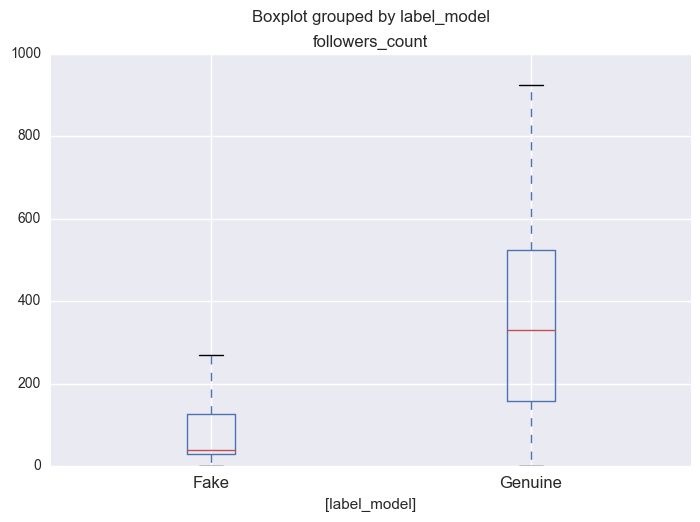
\includegraphics[width =\linewidth]{followers_count.png}
	\end{subfigure}
	~
    \begin{subfigure}[c]{0.3\linewidth}
    	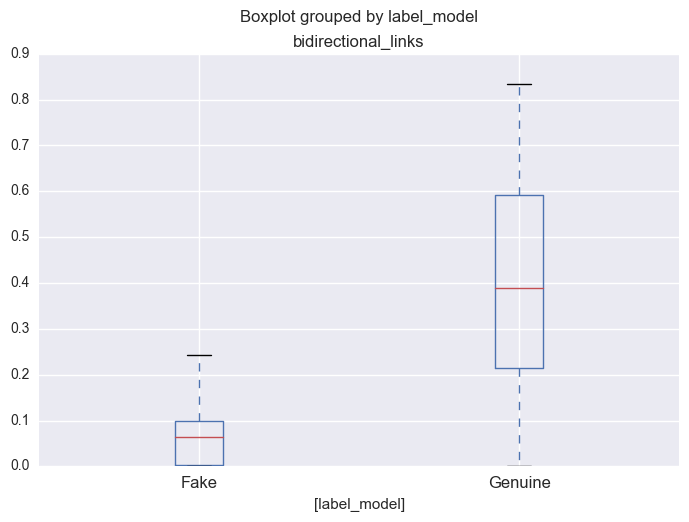
\includegraphics[width =\linewidth]{bidirectional_links.png}
    \end{subfigure}
	~
    \begin{subfigure}[c]{0.3\linewidth}
    	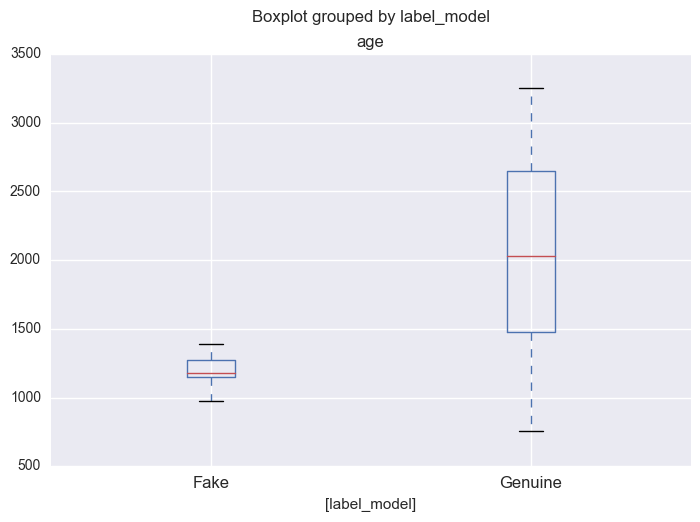
\includegraphics[width =\linewidth]{age.png}
    \end{subfigure}
	~
	\begin{subfigure}[c]{0.3\linewidth}
		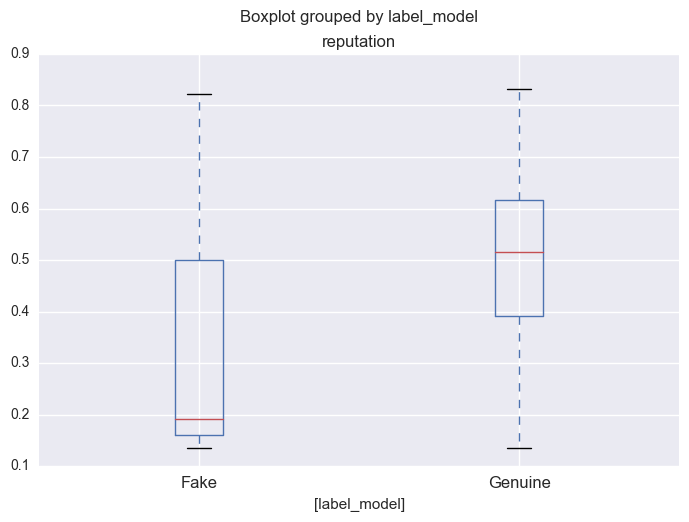
\includegraphics[width =\linewidth]{reputation.png}
	\end{subfigure}
	~
	\begin{subfigure}[c]{0.3\linewidth}
		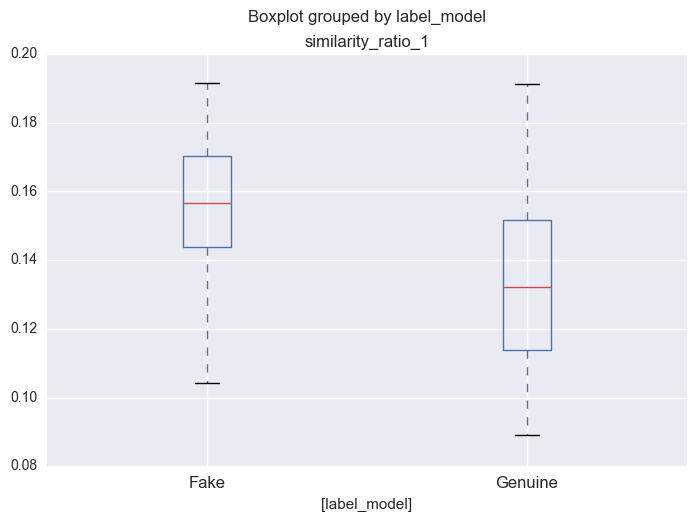
\includegraphics[width =\linewidth]{similarity_ratio_1.png}
	\end{subfigure}
	~
	\begin{subfigure}[c]{0.3\linewidth}
	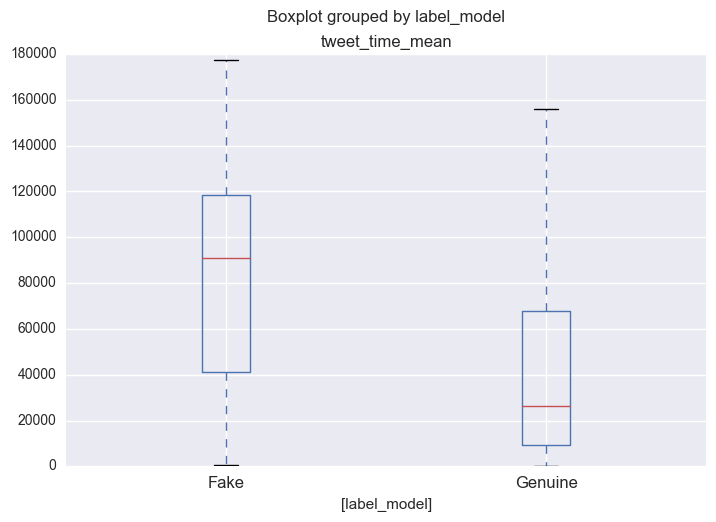
\includegraphics[width =\linewidth]{tweet_time_mean.png}
	\end{subfigure}
	~
	\begin{subfigure}[c]{0.3\linewidth}
		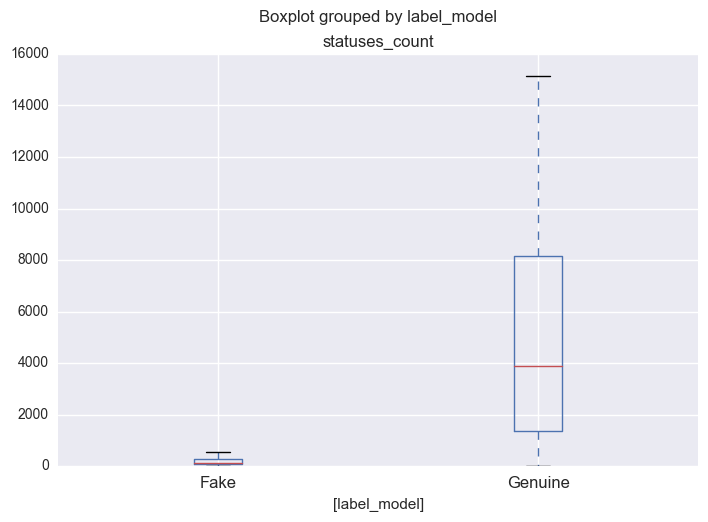
\includegraphics[width =\linewidth]{statuses_count.png}
	\end{subfigure}
	~
	\begin{subfigure}[c]{0.3\linewidth}
		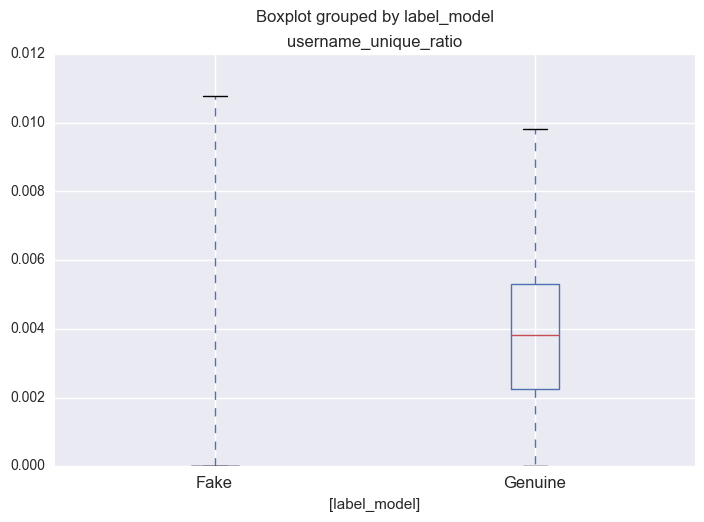
\includegraphics[width =\linewidth]{username_unique_ratio.png}
	\end{subfigure}
	~
	\begin{subfigure}[c]{0.3\linewidth}
	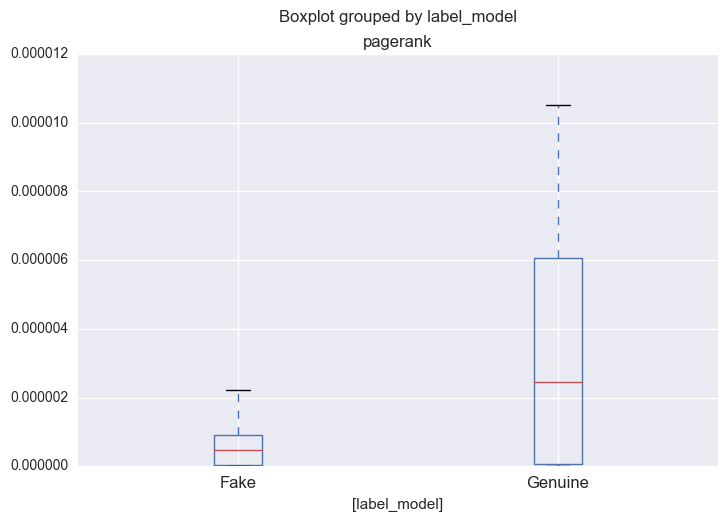
\includegraphics[width =\linewidth]{pagerank.png}
	\end{subfigure}
	\caption{Feature Boxplots of Fake Users and Genuine Users}
	
\end{figure}

\noindent From the plots above, we found the preliminary characteristics of fake/spam users:
\begin{enumerate}
	\item Has a significantly lower number of followers and bidirectional links ratio
	\item The fake account generally gets deleted by Twitter in a much shorter period of time than the genuine ones, which results in a lower score in the age category
	\item Has a lower reputation score
	\item Has a higher tweet similarity ratio and tweet\_time\_mean score, which indicates that these users often produce similar tweet content within a short period of time
	\item Has a significantly lower number of statuses count
	\item Often do not mention other users in their tweets
	\item Has a lower pagerank score
\end{enumerate}

\subsection*{Random Forest}
We applied 47 features on the randomly selected twitter accounts. Then, we use these feature scores and their appropriate labels to build a random forest. This model takes a subset of the datasets and features to build the decision trees. It repeatedly build multiple trees and aggregate the prediction results. \par

\noindent We first randomly chose 70\% of our data as training dataset and 30\% as testing dataset. In order to increase the predictive power and make it easier to train the model, we used the RandomizedSearchCV function in Scikit-learn library to find the best parameters. Table 2 shows the descriptions of the features that we believe can improve the model's overall performance, accuracy and speed. Table 3 displays the optimal parameters and their values found from RandomizedSearchCV for all 4 sample datasets.

\begin{table}[h!]
	\caption{Parameter Descriptions}
	\begin{tabular}{ | l | p{12cm} |}
		\hline
		Parameter & Description  \\
		\hline
		max\_features & The number of features to consider when looking for the best split \\ 
		\hline
		n\_estimators & The number of trees in the forest \\ 
		\hline
		min\_samples\_leaf & The minimum number of samples required to be at a leaf node \\
		\hline
		criterion & The function that measures the quality of a split  \\
		\hline
		random\_state & The random number generator \\ 
		\hline
		class\_weight & A function that  penalizes mistakes in samples of class[i] \\ 
		\hline
	\end{tabular}
\end{table}

\begin{table}[h!]
	\caption{Best Parameters for Random Forest}
	\begin{tabular}{l*{4}{c}r}
		\hline
		Parameters     & Sample\_Data\_1 & Sample\_Data\_2 & Sample\_Data\_3 & Sample\_Data\_4 \\
		\hline
		max\_features & log2 & log2 & log2 & log2  \\
		n\_estimators & 126 & 103 & 180 & 195  \\
		min\_samples\_leaf & 69 & 50 & 69 & 52  \\
		criterion & entropy & gini & gini & gini  \\
		random\_state & 1 & 12 & 15 & 10  \\
		class\_weight & {0:10} & {0:10} & {0:10} & {0:10}  \\
		\hline
	\end{tabular}
\end{table}


\noindent When tuning the parameters, we conducted 5-fold cross validation, in which allows us to randomly partition the training data into 5 equal size subsamples and evaluate the random forest model. We also found the accuracy score, in which calculates the probability that the predicted labels match with the true labels. From table 4, we can see that the cross validation scores for Sample Datasets\_1 to 3 are ranged from 0.95 and 0.98. However, the score for Sample\_Datasets\_4 is much lower than the rest. We believe the distribution of fake and genuine accounts in these datasets contribute to the difference in scores. For the first three sample datasets, we mimic the true distribution in reality, in which 10.78\% of them are fake and the rest are genuine. However, the genuine to fake ratio of sample dataset\_4 is 3:1. \par

\begin{table}[h!]
	\caption{Cross Validation and Accuracy Score}
	\centering
	\begin{tabular}{p{3cm} |p{3.5cm}|p{3.5cm}|p{3.5cm}}	
		\hline
		Datasets & Cross\_Validation
		Score\_Mean    & Cross\_Validation
		Score\_Standard Deviation
		& Metrics\_Accuracy
		Score\\
		\hline
		Sample\_Data\_1 & 0.942    &0.014 & 0.942\\
		\hline
		Sample\_Data\_2 & 0.961    &0.008 & 0.961\\
		\hline
		Sample\_Data\_3 & 0.964    &0.009 & 0.964\\
		\hline
		Sample\_Data\_4 & 0.913    &0.014 & 0.913\\
		\hline
	\end{tabular}
\end{table}

\noindent After finding the best parameters, we used them to fit the model on the training dataset and illustrated the importance of each feature ratio in predicting the correct twitter account label with barplot. Figure 2 shows the total number of favorites that a particular user gets (favorites\_count) is the most effective predictor for sample dataset (1-3) because this feature is based on how the third party (other twitter users) responds to the content that this particular user has produced. However, if 25\% of our sample dataset are fake accounts, the website ratio has the highest predictive power because a high score is a good indicator of fake account.  

\begin{figure}[h!]
	\centering
	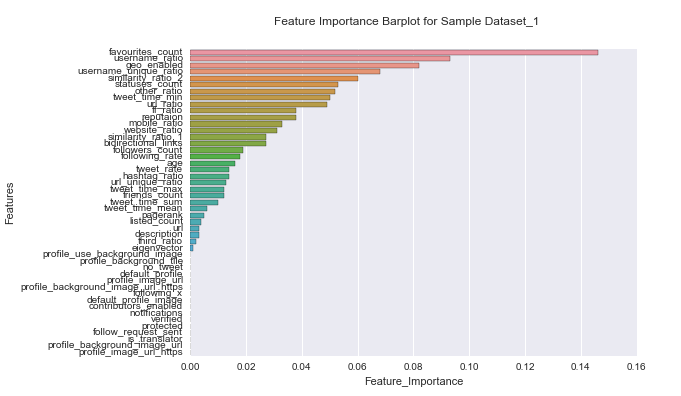
\includegraphics[scale=0.7]{feature_1}
	\caption{Feature Importance}
\end{figure}

\begin{figure}[h!]
	\centering
	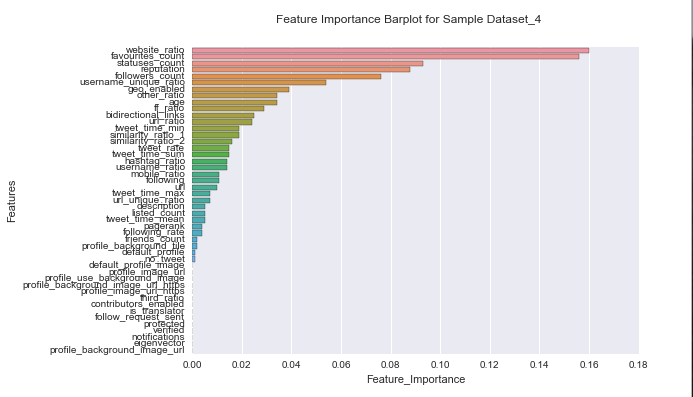
\includegraphics[scale=0.7]{feature_4}
	\caption{Feature Importance}
\end{figure}

\noindent Lastly, we used confusion matrix to check the accuracy of the random forest model. In order to better visualize and interpret the results, we used the normalized confusion matrix to make sure that the ratio is at the same scale. Figure 4 illustrates the fake accounts have higher prediction accuracy score in general, in which indicates that the model did a better job in predicting the fake accounts. We got very similar confusion matrix scores for all the datasets. 

\begin{figure}[h!]
	\centering
	\begin{subfigure}{0.45\linewidth}
		\centering
		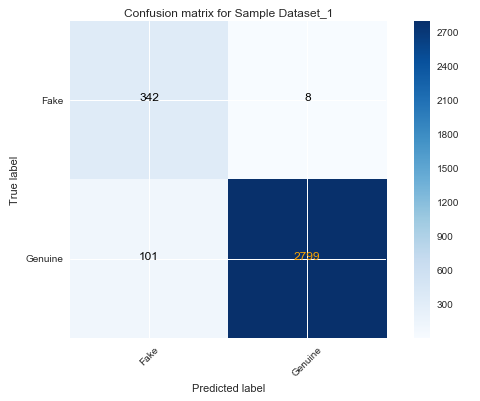
\includegraphics[width =\linewidth]{matrix_1}
		\subcaption{Without Normalization}
	\end{subfigure}%
	\begin{subfigure}{0.45\linewidth}
		\centering
		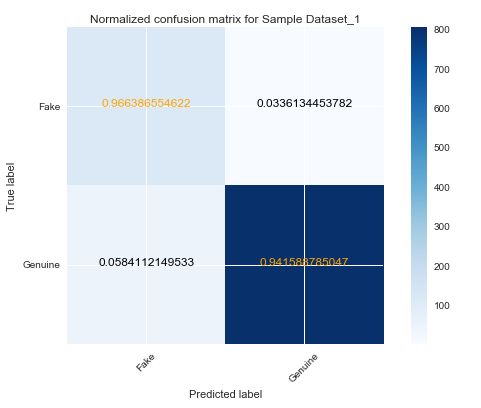
\includegraphics[width =\linewidth]{matrix_nor_1}
		\subcaption{With Normalization}
	\end{subfigure}
	\caption{Confusion Matrix for Sample 1}
\end{figure}


\subsection*{Logistic Regression}
First, we ran a default logistic regression model with the cost parameter $C=1$. The accuracy score is around 90.92\%. However, the probability for identifying fake accounts given the true fake label is around 35.52\%. The unbalanced dataset explains the reason behind the high overall accuracy score but low for individual category. Therefore, we needed to tune our parameters so that it can accurately predict both account types with low prediction error. 

\noindent We used the GridSearchCV function in the Scikit-learn library to find the best parameters for logistic regression. We tuned the following parameters: C, penalty and class\_weight. C is the inverse of regularization strength, which is the parameter of penalty. The settings for penalty are L1 and L2. We also adjusted the class weight for the fake twitter accounts to penalize the error for identifying fake accounts. In other words, it costs more to make a wrong prediction on a fake account, which leads to a higher accuracy in predicting this particular category. 

\begin{table}[h!]
	\captionof{table}{Best Parameters of Logistic Regression} \label{tab:title} 
	\begin{center}
		\begin{tabular}{rrrrrr}
			\hline
			& Cost & Penalty & Class weight & Mean validation score & Accuracy score\\
			\hline
			Sample 1 & 1.0 & l1 & 3 & 0.964 & 0.962\\
			Sample 2 & 100 & l1 & 3 & 0.960 & 0.971\\
			Sample 3 & 10  & l1 & 3 & 0.970 & 0.965\\
			\hline
		\end{tabular}
	\end{center}
\end{table}

\noindent After tuning the parameters and fitting them on the model, we improved the overall accuracy to 95.38\% with the probability of predicting the fake accounts correctly equals to 88.16\%.

\subsection*{Support Vector Machine}
\subsubsection*{rbf SVM}
In rbf kernel SVM, our objective is to find the best cost parameter C, gamma $\gamma$ in kernel function and class weight, in which penalizes more on the missclassification of fake users. After conducting the gridsearch with 5-fold cross-validation, most parameter combinations found yielded to similar mean validation scores. The following table describes the scores for the best parameters found for all the sample datasets. 

\begin{table}[h!]
	\captionof{table}{Best Parameters of rbf SVM} \label{tab:title} 
	\begin{center}
		\begin{tabular}{rrrrrr}
			\hline
			& Cost & $\gamma$ & Class weight & Mean validation score & Accuracy score\\
			\hline
			Sample 1 & 0.01 & 0.01 & 5 & 0.893 & 0.890\\
			Sample 2 & 0.01 & 0.001 & 3 & 0.969 & 0.893\\
			Sample 3 & 0.01 & 0.01 & 5 & 0.893 & 0.890\\
			\hline
		\end{tabular}
	\end{center}
\end{table}

\noindent The confusion matrix shows that all the accounts in the test data are labeled as genuine, indicating that rbf SVM kernel fails to discriminate the small-proportion fake users from the large number of genuine accounts. Although the general accuracy score is acceptable, the model is not useful for detection purpose.
\begin{figure}[h!]
	\centering
	\begin{subfigure}[c]{0.45\linewidth}
		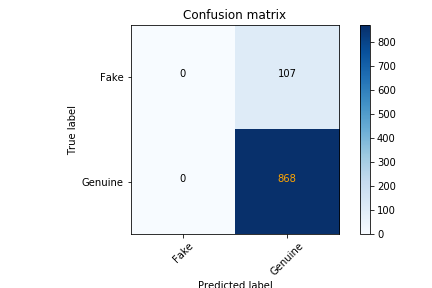
\includegraphics[width =\linewidth]{rbf_svc_confm_11.png}
	\end{subfigure}
	~
	\begin{subfigure}[c]{0.45\linewidth}
		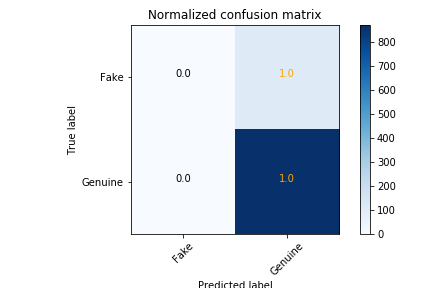
\includegraphics[width =\linewidth]{rbf_svc_confm_12.png}
	\end{subfigure}
	\caption{Confusion Matrix of rbf SVM}
\end{figure}


\subsubsection*{Linear SVM}
The linear SVM model finds the best norm used in the penalization, cost parameter C and class weight. After conducting cross validation, we found the best set of parameters as describes below.

\begin{table}[h!]
	\captionof{table}{Best Parameters of Linear SVM} \label{tab:title} 
	\begin{center}
		\begin{tabular}{rrrrrr}
			\hline
			& Cost & Penalty & Class weight & Mean validation score & Accuracy score\\
			\hline
			Sample 1 & 100 & l1 & 3 & 0.960 & 0.960\\
			Sample 2 & 100 & l1 & 3 & 0.969 & 0.960\\
			Sample 3 & 100 & l1 & 3 & 0.968 & 0.963\\
			\hline
		\end{tabular}
	\end{center}
\end{table}

\noindent The confusion matrix of sample dataset 3 has the lowest TP (The probability of predicting fake user given the true label is fake user). The TP rate is approximately 91\% and FP rate is around 3\%. Although there is a process to appeal, we still want relatively low FP rate since it is possible to lose a genuine user when it is classified as fake account.

\begin{figure}[H]
	\centering
	\begin{subfigure}[c]{0.45\linewidth}
		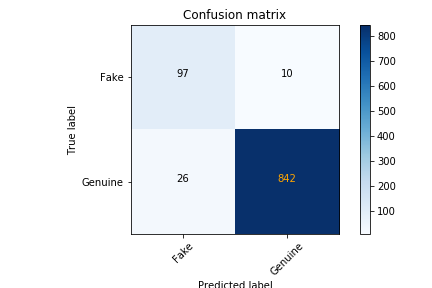
\includegraphics[width =\linewidth
		]{linear_svc_confm_31.png}
	\end{subfigure}
	~
	\begin{subfigure}[c]{0.45\linewidth}
		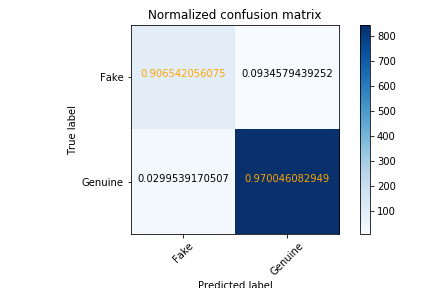
\includegraphics[width =\linewidth]{linear_svc_confm_32.png}
	\end{subfigure}
	\caption{Confusion Matrix of Linear SVM}
\end{figure}





\section*{FUTURE DISCUSSION}
Here are some possible directions that we are considering for the next step:

\noindent 1. Create more features in predicting the account type\\
2. Further evaluate the models that we built and use methods to reduce noise and errors\\
3. Investigate  more on other models that we can potentially use\\
4. Create an interactive platform to allow the Twitter users to use our predictive models\\

\newpage
\large\textbf{Appendix} 
\section*{Reflection}
Overall, we had successfully accomplished the goal of our project, in which allows the Twitter users to identify whether the account is fake or genuine using Random Forest, Logistic Regression and Support Vector Machine. We were unable to analyze the fake users' behaviors on the trend topics due to the time constraint. Each group member was assigned to build different features and predictive models. All of us had contributed equally. We met regularly to check on each other's progress and discuss the problems that we had encountered. Since each of us has very different levels of skill sets and knowledge, it was challenging to include and implement everyone's initial ideas. However, we were able to compromise and find common interests through discussions. Originally, we wanted to analyze all the tweets that the user has posted and create a network to illustrate the following relationship for the selected users. However, the Twitter API has set limit on the amount of info that we could get. Therefore, we only downloaded the maximum number of tweets that we were allowed. We also only calculated two statistics that are associated with the graph due to the time constraint. In addition, we originally planned to build features on predicting the twitter account types from the scratch. However, we had realized that it is important to conduct research on previous studies and use them as references, in which saves us time and helps increase the effectiveness of the features. \\

\noindent As the project progressed, we narrowed down the models that we wanted to build and tried to understand the math and concepts behind them, We learned that it is important to create a feasible time-line for any project because it is often easy to overestimate the amount of work that we think we can accomplish. In addition, we needed to understand the context of the data, the intuitions behind the models and how our analysis can help answer the questions that we wanted to solve. Most importantly, we gained a better understanding of working on a statistical project and the importance of effective communication and teamwork. \\

\newpage
\section*{Codes}
SVM.py - builds svm model\\
random\_forest.py - builds random forest model\\
t\_analysis.py - calculates tweet analysis ratios\\
similarity\_1.py - calculates tweet similarity ratio 1\\
similarity\_2.py - calculates tweet similarity ratio 2\\
tweet\_ratio.py - creates a csv file that contains the tweet analysis ratios\\
sim\_1\_df.py - creates a csv file for storing the tweet similarity ratio 1 result\\
sim\_2\_df.py - creates a csv file for storing the tweet similarity ratio 2 result\\
combine\_df.py - combines all the feature results into a dataframe\\
tweet\_time\_diff.py - calculates the time difference between two consecutive tweets\\


\newpage
\section*{Reference}
\begin{lstlisting}
[1]O.Varol, E.Ferrara, C.A.Davis, F.Menczer, and A.Flammini. Online Human-Bot Interactions: Detection, Estimation, and Characterization
[2] F. Benevenuto, G. Magno, T. Rodrigues, and V. Almeida. Detecting Spammers on Twitter. In Collaboration, Electronic messaging, Anti-Abuse and Spam Confference.
[3] K. Lee, J. Caverlee, and S. Webb. Uncovering Social Spammers: Social Honeypots Machine Learning. In ACM SIGIR Conference (SIGIR), 2010.
[4] G. Stringhini, S. Barbara, C. Kruegel, and G. Vigna. Detecting Spammers On Social Networks. In Annual Computer Security Applications Conference (ACSAC’10), 2010.
[5] A. Wang. Don’t follow me: spam detecting in Twitter. In Int’l Conferene on Security and Cryptography (SECRYPT), 2010.
[6] G. Stringhini, C. Kruegel, G. Vigna Detecting Spammers on Social Networks
[7] C. Yang, R. Harkreader, and G. Gu. Empirical evaluation and new design for fighting evolving Twitter spammers. I.
[8] N. de Freitas. "Machine learning - Random forests." Online video clip. YouTube. YouTube, 21 Feb 2013
[9] D.Jurafsky, J.H. Martin. "Speech and Language Processing"
 
\end{lstlisting}
\end{document} 